\documentclass[12pt,utf8,notheorems,compress,t]{beamer}
\usepackage{etex}

\usepackage[english]{babel}

\usepackage{mathtools}
\usepackage{booktabs}
\usepackage{array}
\usepackage{ragged2e}
\usepackage{multicol}
\usepackage{tabto}
\usepackage{xstring}
\usepackage{mathtools}
\usepackage{tikz}
\usetikzlibrary{calc,shapes.callouts,shapes.arrows}

\usepackage[protrusion=true,expansion=true]{microtype}

\newcommand{\E}{\mathcal{E}}
\newcommand{\F}{\mathcal{F}}
\renewcommand{\O}{\mathcal{O}}
\newcommand{\K}{\mathcal{K}}
\newcommand{\defeq}{\vcentcolon=}
\newcommand{\defeqv}{\vcentcolon\equiv}
\newcommand{\Sh}{\mathrm{Sh}}
\renewcommand{\_}{\mathpunct{.}}
\newcommand{\?}{\,{:}\,}

\setlength\parskip{\medskipamount}
\setlength\parindent{0pt}

\title{Using the internal language of toposes in algebraic geometry}
\author{Ingo Blechschmidt}
\date{November 27th, 2015}

\usetheme{Warsaw}
\usecolortheme{seahorse}
%\usefonttheme{default}?
%\usepackage{kurier}?
\usefonttheme{serif}
%\usepackage{libertine}?
\usepackage{mathpazo}
\useinnertheme{rectangles}

\setbeamertemplate{blocks}[rounded][shadow=false]

\newenvironment{changemargin}[2]{%
  \begin{list}{}{%
    \setlength{\topsep}{0pt}%
    \setlength{\leftmargin}{#1}%
    \setlength{\rightmargin}{#2}%
    \setlength{\listparindent}{\parindent}%
    \setlength{\itemindent}{\parindent}%
    \setlength{\parsep}{\parskip}%
  }%
  \item[]}{\end{list}}

\newcommand{\pointthis}[2]{%
        \tikz[remember picture,baseline]{\node[anchor=base,inner sep=0,outer sep=0]%
        (#1) {#1};\node[overlay,rectangle callout,%
        callout relative pointer={(-0.2cm,0.8cm)},fill=blue!20] at ($(#1.north)+(1.8cm,-1.4cm)$) {#2};}%
        }%

\setbeamertemplate{frametitle}[default][colsep=-2bp,rounded=false,shadow=false,center]

\setbeamertemplate{headline}{}
\setbeamertemplate{navigation symbols}{}

\newcommand{\floatbox}[3]{%
  \raisebox{0pt}[0pt][0pt]{%
    \begin{picture}(0,0)(#1,#2)#3\end{picture}\leavevmode%
  }%
}

\newcommand{\backupstart}{
  \newcounter{framenumberpreappendix}
  \setcounter{framenumberpreappendix}{\value{framenumber}}
}
\newcommand{\backupend}{
  \addtocounter{framenumberpreappendix}{-\value{framenumber}}
  \addtocounter{framenumber}{\value{framenumberpreappendix}} 
}

\setbeamertemplate{footline}{%
  \begin{beamercolorbox}[wd=\paperwidth,ht=2.5ex,dp=1.25ex,right,rightskip=1mm,leftskip=1mm]{frametitle right}
    {\quad} \inserttitle \hfill \insertauthor \quad
    \insertframenumber\,/\,\inserttotalframenumber {\quad}
  \end{beamercolorbox}}

\newcommand{\hil}[1]{{\usebeamercolor[fg]{item}{\textbf{#1}}}}

\IfSubStr{\jobname}{\detokenize{nonotes}}{
  \setbeameroption{hide notes}
}{
  \setbeameroption{show notes}
}
\setbeamertemplate{note page}[plain]

\begin{document}

\begin{frame}[c]
  \centering
  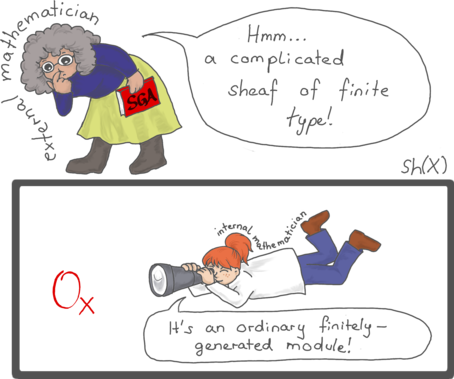
\includegraphics[scale=0.3]{external-internal-small.png}
  \medskip

  \hil{Using the internal language of toposes in \\ algebraic geometry}
  \medskip

  \scriptsize
  Ingo Blechschmidt \\
  University of Augsburg
  \medskip

  Topos à l'IHES \\
  November 27th, 2015
  \par
\end{frame}

\frame[t]{\frametitle{Outline}\scriptsize\begin{itemize}\item[]\tableofcontents\end{itemize}}

\note{\justifying\fontsize{8pt}{9.6}\selectfont
  \begin{center}\large\textbf{Abstract}\end{center}

  \begin{changemargin}{2.5em}{2.5em}
    We describe how the internal language of certain
    toposes, the associated petit and gros Zariski toposes of a scheme, can be
    used to give simpler definitions and more conceptual proofs of the basic
    notions and observations in algebraic geometry.
    % This is useful for studying schemes from a local or relative point of view.

    The starting point is that, from the internal point of view, sheaves of rings
    and sheaves of modules look just like plain rings and plain modules.
    In this way, some concepts and statements of scheme theory can be reduced to
    concepts and statements of intuitionistic linear algebra.

    Furthermore, modal operators can be used to model phrases such as ``on a
    dense open subset it holds that'' or ``on an open neighbourhood of a given
    point it holds that''. These operators define certain subtoposes; a
    generalization of the double-negation translation is useful in order to
    understand the internal universe of those subtoposes from the internal point
    of view of the ambient topos.

    A particularly interesting task is to internalize the
    construction of the relative spectrum, which, given a quasicoherent sheaf of algebras
    on a scheme~$X$, yields a scheme over~$X$. From the internal point of
    view, this construction should simply reduce to an intuitionistically sensible
    variant of the ordinary construction of the spectrum of a ring, but it turns
    out that this expectation is too naive and that a refined approach is
    necessary.
  \end{changemargin}
}


\section{Basic examples}

\begin{frame}[c]\frametitle{Exact sequences}
  \centering
  \begin{minipage}{0.75\textwidth}
    \begin{exampleblock}{}
      \justifying
      Let~$0 \to M' \to M \to M'' \to 0$ be a short exact sequence of
      modules. If~$M'$ and~$M''$ are finitely generated, so is~$M$.
    \end{exampleblock}
  \end{minipage}
  \medskip

  \scalebox{3}{$\Downarrow$}

  \begin{minipage}{0.75\textwidth}
    \begin{exampleblock}{}
      \justifying
      Let $0 \to \F' \to \F \to \F'' \to 0$ be a short exact sequence
      of~$\O_X$-modules. If~$\F'$ and~$\F''$ are locally of finite type, so
      is~$\F$.
    \end{exampleblock}
  \end{minipage}
  \par
\end{frame}

\begin{frame}[c]\frametitle{Local freeness}
  \centering
  \begin{minipage}{0.70\textwidth}
    \begin{exampleblock}{}
      \justifying
      Any finitely generated vector space does \emph{not not} possess a basis.
    \end{exampleblock}
  \end{minipage}
  \medskip

  \scalebox{3}{$\Downarrow$}

  \begin{minipage}{0.70\textwidth}
    \begin{exampleblock}{}
      \justifying
      Any sheaf of modules of finite type on a reduced scheme is locally free
      \emph{on a dense open subset}.
    \end{exampleblock}
  \end{minipage}
  \par
\end{frame}

\begin{frame}\frametitle{Further examples}
  Let~$X$ be a scheme. Internally to~$\Sh(X)$,
  \begin{itemize}
    \item any non-invertible element of~$\O_X$ is nilpotent,
    \item $\K_X$ is simply the total quotient ring of~$\O_X$,
    \item $\dim \O_X \leq n$ holds if and only if~$\dim X \leq n$.
  \end{itemize}
\end{frame}


\section{The $\Diamond$-translation}

\newcommand{\idiamond}{{\usebeamercolor[fg]{item}{\boldsymbol{\Diamond}}}}
\newcommand{\gdiamond}[1]{\textcolor{gray}{\boldsymbol{\Diamond}(}#1\textcolor{gray}{)}}

\begin{frame}\frametitle{The $\Diamond$-translation}
  Let~$\E_\Diamond \hookrightarrow \E$ be a subtopos given by a \pointthis{local
  operator}{$\Diamond : \Omega_\E \to \Omega_\E$}~$\Diamond$. Then
  \[ \E_\Diamond \models \varphi \qquad\text{iff}\qquad
    \E \models \varphi^\Diamond\only<2->{.}\only<1>{,}\]
  \only<1>{where the translation~$\varphi \mapsto \varphi^\Diamond$ is given by:
  \begin{align*}
    (s = t)^\Diamond &\defeqv \idiamond(s=t) \\
    (\varphi \wedge \psi)^\Diamond &\defeqv \gdiamond{\varphi^\Diamond \wedge \psi^\Diamond} \\
    (\varphi \vee \psi)^\Diamond &\defeqv \idiamond(\varphi^\Diamond \vee \psi^\Diamond) \\
    (\varphi \Rightarrow \psi)^\Diamond &\defeqv \gdiamond{\varphi^\Diamond \Rightarrow \psi^\Diamond} \\
    (\forall x\?X\_ \varphi(x))^\Diamond &\defeqv \gdiamond{\forall x\?X\_ \varphi^\Diamond(x)} \\
    (\exists x\?X\_ \varphi(x))^\Diamond &\defeqv \idiamond(\exists x\?X\_ \varphi^\Diamond(x))
  \end{align*}}

  \only<2->{
    Let~$X$ be a scheme. There are choices for~$\Diamond$ such that~$\Sh(X)
    \models \Diamond\varphi$ means that~$\varphi$ holds on \ldots
    \begin{itemize}
      \item \ldots{} a dense open subset.
      \item \ldots{} a given open subset~$U$.
      \item \ldots{} an open subset containing a given closed subset~$A$.
      \item \ldots{} a neighbourhood of a given point~$x \in X$.
    \end{itemize}

    \pause
    Can tackle the question~``$\varphi^\Diamond \stackrel{?}{\Rightarrow} \Diamond\varphi$'' logically.
  }
\end{frame}


\section{Quasicoherence}

\begin{frame}\frametitle{Quasicoherence}
  Let~$X$ be a scheme. Let~$\F$ be an~$\O_X$-module.

  Then~$\F$ is quasicoherent
  if and only if, internally to~$\Sh(X)$,
  \begin{quote}\textnormal{$\F[f^{-1}]$ is a $\Diamond_f$-sheaf for any~$f : \O_X$, \\[0.3em]
  \qquad\qquad where~$\Diamond_f\varphi \defeqv (\text{$f$ invertible} \Rightarrow \varphi)$.}
  \end{quote}
  \pause

  In particular: If~$\F$ is quasicoherent, then internally
  \[ (\text{$f$ invertible} \Rightarrow s = 0) \Longrightarrow
    \bigvee_{n \geq 0} f^n s = 0 \]
  \vspace*{-1.5em}\par%
  for any~$f : \O_X$ and~$s : \F$.
\end{frame}


\section{The relative and internal spectrum}

\begin{frame}\frametitle{}
\end{frame}

\end{document}
